\scanpage{12}
\mspage{9}
Alors on voit que
\[
L^{n-i+\alpha}q_{i\alpha}:M^i\unsure{-|\longrightarrow}M^{2n-i+2\alpha}
\]
est nul sur les $L^{\alpha'}P^{i-2\alpha'}$ pour $\alpha'\neq\alpha$, et que sur $L^\alpha P^{i-2\alpha}$, \deleted{\unsure{il}} son composé avec
\[
P^{i-2\alpha}\xrightarrow{L^\alpha}L^\alpha P^{i-2\alpha}
\]
n'est autre que l'isom
\[
L^{\unsure{n-i-2\alpha|n-i+2\alpha}}:P^{i-2\alpha}\unsure{\Rightarrow|\longrightarrow}L^{n-i+2\alpha}P^{i-2\alpha}\subset M^{2n-i+2\alpha}.
\]
Il s'ensuit aussitôt que
\[
\pi_{i,\alpha}=L^\alpha w_{i-2\alpha}L^{n-i+\alpha}q_{i\alpha}=L^\alpha w_{i-2\alpha}L^{n-i+\alpha}(1-\sum_{\alpha'>\alpha}\pi_{i,\unsure{\alpha'}}
\tag{6.9}
\]
ce qui donne bien $\pi_{i\alpha}\in\mathcal E$. \deleted{Cela prouve (iv).}
Si $i<n$, il faut, \unsure{égalt} $\pi_{2n-i,\alpha}\in\mathcal E$. On
\deleted{Reste à prouver \inserted{(iii)} $\Lambda\in\mathcal E$. Il suffit de \deleted{\unsure{prendre}} \unsure{poser}
\[
q_{2n-i,\alpha}=1-\sum_{\alpha'>\alpha}\pi_{2n-i,\alpha'}
\]
et on voit alors que
\[
\deleted{\unsure{L^{n-i+\alpha}}}L^\alpha q_{2n-i,\alpha}:M^{2n-i}\unsure{-|\longrightarrow}M^{2n-i+2\alpha}
\]}
le déduit p. ex. de la formule
\[
\pi_{2n-i,\alpha}=L^{n-i}\pi_{i,\alpha}w_i\deleted{\unsure{\pi_{2n-i}}}
\tag{6.10}
\]
Cela prouve \inserted{\figure{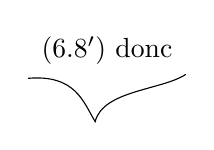
\begin{tikzpicture}[x=1cm,y=1cm]
\node at (0,.25) {$(6.8')$ donc};
\draw (-1,-.1) .. controls (-.4,-.05) and (-.3,-.4) .. (-.15,-.65) .. controls (-.05,-.25) and (.7,-.25) .. (1,-.05);
\end{tikzpicture}}} (iv). Reste : prouver (iii) $\Lambda\in\mathcal E$.

Comme on a
\[
\Lambda=\sum_{j,\alpha\,\deleted{\unsure{j\leq n}}}\deleted{\unsure{\Lambda}}\Lambda\pi_{j,\alpha}\quad\deleted{\unsure{+\sum_{0\leq i\leq n}\pi_{i,0}\Lambda}}
\tag{6.11}
\]
il suffit de prouver que $\Lambda\pi_{i\alpha}\deleted{\unsure{\Lambda\pi_{i,\alpha}|\pi_{i,\alpha}}}\in\mathcal E$.
\mspage{11}
